\documentclass[12pt, a4paper]{article}
\usepackage[T1]{fontenc}
\usepackage[utf8]{inputenc}
\usepackage{graphicx, textcomp, gensymb, tabularx, booktabs, wrapfig, indentfirst, amsmath, geometry, amssymb, caption}
\graphicspath{{fig/}}
\usepackage[backend = biber]{biblatex}
\newgeometry{tmargin=2cm, bmargin=2cm, lmargin=2cm, rmargin=2cm}
\renewcommand{\figurename}{ryc.}

\begin{document}

\title{
	Identification the presence of metastases from histopathology images
}
	
\author{
	Maciej Draguła
}

\date{5 February 2020}


\maketitle

\section{Introduction}

\subsection*{What is the problem?}
\noindent
The goal is to identify the presence of metastases from 96 x 96px digital histopa\-thology images so this is a binary image classification problem. One of possible challanges is that the metastases can be as small as single cells in a large area of tissue. The problem is taken from Kaggle.

\begin{figure}[ht]
	\centering
	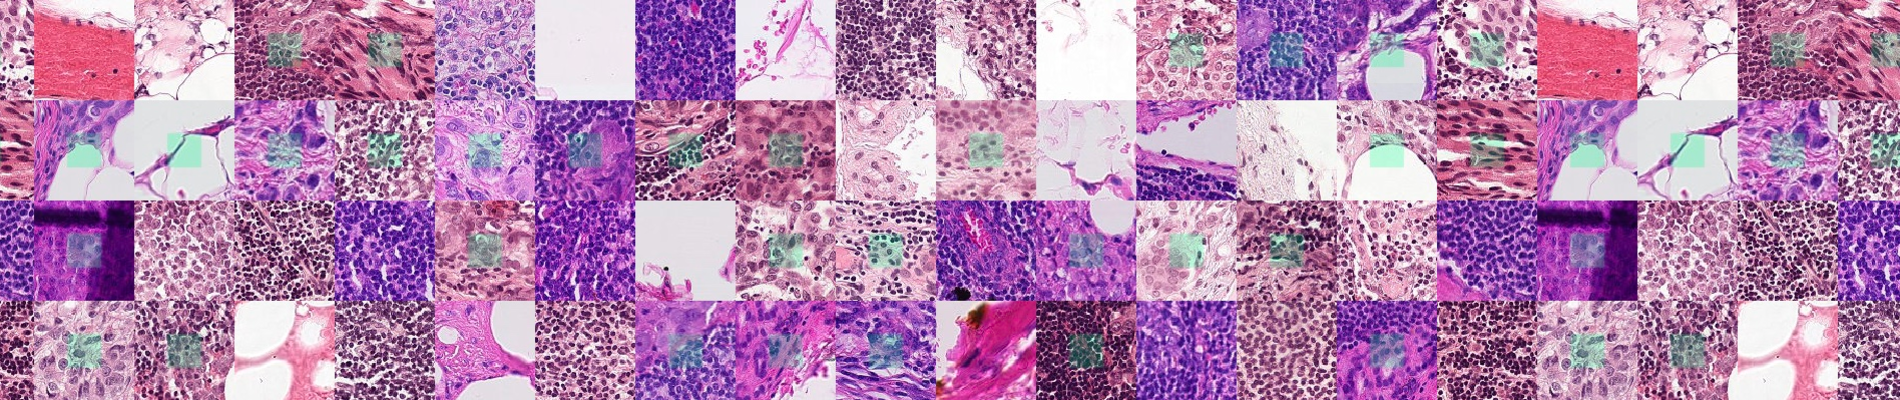
\includegraphics[width = 16cm]{header.png}
\end{figure}

\subsection*{What is exactly on the images?}

\noindent
The histopathological images are microscope images of lymph nodes that were stained with hematoxylin and eosin (H\&E). H\&E allows to detect various objects like nuclei (blue), cytoplasm and extracellular parts (both red and pink). Hematoxylin binds to negatively charged substances like nucleic acids and pink eois to positively charged substances like amino acids side chains which makes visible difference on the image. According to American Cancer Society lymph nodes are the first place a breast cancer is likely to spread.

\begin{figure}[ht]
	\centering
	\includegraphics[width =5cm]{roc.png}
\end{figure}

\subsection*{How to find the best solution?}

\noindent
In binary classification one of the good metric is area under the ROC curve. The ROC curve is a plot of True positive rate against False positive rate at various thresholds. The area under the curve is equal to the probability that a classifier will rank a randomly chosen positive instance higher than a randomly chosen negative one so the bigger the area under the curve the better classifier we have. You can see an example of almost perfect classifier below.

\section{Description of data}

\subsection*{What kind of data do we have?}

\noindent
About 220k training images and 57k evaluation images.  We are not going to use evaluation images because the contest is over and we just want to test performance of models. The dataset is a subset of PCam dataset. 

\noindent
A positive labels means that that there is a least one pixel of tumour tissue in the center region (32 x 32px) of the image. Because tumour tissue in the outer region does not influence the label, it might be a good idea to crop the images to center region (this means that negatively labelled image could contain metastases in the outer region). We decided to focus on 48 x 48px center region however other crops were not investigated.

\noindent
It is easy to see that the training set is not balanced. The ratio is close to 60/40 meaning that there are more negative images.

\subsection*{Understanding data}

\noindent
Lymph node metastases features are described in very complicated way but to simplify: irregular nuclear shapes, sizes or staining shades can indicate metastases. The features might be very subtle thus the problem of classifying metastases is not an easy task for a specialist and extremely hard for an untrained eye like mine. See the example images below with highlighted center areas.

\begin{figure}[ht]
	\centering
	\includegraphics[width =16cm]{scans.png}
\end{figure}

\section{Feature engineering}

\subsection*{Color channels}

\noindent
As mentioned before it is hard to describe useful features but let's do some feature engineering on each channel: red, green and blue. First let's take a look how looks the distribution of colors in each class.

\begin{figure}[ht]
	\centering
	\includegraphics[width =16cm]{color_channels.png}
\end{figure}

\noindent
Now we can clearly spot the difference between classes. Positive samples usually have darker colors (remember: 0 is black, 255). The peaks of distributions from first row are on the left-hand side of peaks from second row. Interesting fact is that many white spots appear in both classes. You can notice a very high value for 255 in blue channel. It might be an artefact which we may need to deal with later. To make sure that negative samples seems to consist of brighter colors than negative samples let's take a look on mean image brightness.

\begin{figure}[ht]
	\centering
	\includegraphics[width =16cm]{brightness.png}
\end{figure}

\noindent
Here we can also see that distribution of mean brightness for positive samples tends to be unimodal with the peak around 160. Whereas for negative samples, it seems to behave like bimodal distribution with peaks in 140 and 220.

\section{k-Nearest Neighbours}

\noindent
At very beginning let's check very naive algorithm - kNN. Because the data set is large and because of RAM limitation we will use on 20k first images and split them in ratio 80:20. See blow the ROC curves for each for each k to see the quality of classifiers. The result is not unexpected. The space is huge so kNN cannot fit correctly and works like random classifier.

\begin{figure}[ht]
	\centering
	\includegraphics[width =16cm]{roc_knn.png}
\end{figure}

\newpage
\section{Convolutional Neural Net}

\subsection*{Model description}
\noindent
The model for this problem will be convolutional neural net using ReLU as an activation function with batch normalization, max pooling and dropouts. Below you can find an architecture of the net.
\begin{itemize}
	\item Convolution layer ({32, 64, 128} filters, 3 x 3 kernel)
	\item Batch normalization layer
	\item Activation layer (ReLU)
	\item Convolution layer ({32, 64, 128} filters, 3 x 3 kernel)
	\item Batch normalization layer
	\item Activation layer (ReLU)
	\item Max pooling layer (2 x 2)
	\item Dropout layer
\end{itemize}
(This block is repeated three times with size of filters given in curly brackets). At the end an output will be flatten and full connected to 256 neurons and finally converted to values from 0 to 1 using sigmoid.
\begin{itemize}
	\item Flatten layer
	\item Fully conected layer (256)
	\item Batch normalization layer
	\item Activation layer (ReLU)
	\item Dropout layer
	\item Fully conected layer (1) with sigmoid
\end{itemize}

\subsection*{Training and validation}
\noindent
The model was compiled with Adam optimizer and binary cross-entropy as loss function. This time we use full dataset and again we split the data using 80\% for training and 20\% for validation.

\noindent
We decided to set batch size on 50 which means that the network will process 50 images at ones. We also added reshuffling the data between the epochs which may improve the outcome.

\noindent
Finally we get $ 86\% $ accuracy on training set and $ 83.8\% $ on test set. You can see the ROC curve below. It is not sure why it has such shape with one sharp point.

\begin{figure}[ht]
	\centering
	\includegraphics[width =6cm]{roc_cnn.png}
\end{figure}

\section{Neural Architecture Search}

\subsection*{What is NAS?}
\noindent
Neural Architecture Search (NAS) is the process of automating architecture engineering i.e. finding the design of our machine learning model. Where we need to provide a NAS system with a dataset and a task (classification, regression, etc), and it will give us the architecture. And this architecture will perform best among all other architecture for that given task when trained by the dataset provided. NAS can be seen as a subfield of AutoML and has a significant overlap with hyperparameter optimization. To understand NAS we need to look deeply into what it is doing. It finds an architecture from all possible architectures by following a search strategy that will maximize the performance. The following figure summarizes the NAS algorithm.
\begin{figure}[ht]
	\centering
	\includegraphics[width=12cm]{nas.png}
\end{figure}

\noindent
Search space defines what neural architecture a NAS approach might discover in principle. The search strategy and performance estimation can be solved with RL. Reinforcement learning is the problem faced by an agent that must learn behaviour through trial and error interactions with a dynamic environment to maximize some reward. In the case of NAS, the agent produces the model architecture. Then the model is trained on the dataset and the performance of the model on the validation data is taken as a reward.

\subsection*{Model description}
\noindent
We decided to use built-in NASNetMobile. The output from the net is passed through GlobalAveragePooling to fully connected layer with sigmoid used as an activation function.

\subsection*{Training and validation}
\noindent
Again we will use Adam as optimizer and binary cross entropy as a loss function. The data is is again split between training and validation in ratio 80:20.

\noindent
At the end we have accuracy on training set $ 93.2\% $ and $ 88.9 \% $ accuracy.

\section{Conclusions and further work}

\noindent
Needless to say, that classic algorithm like kNN is not enough efficient to process this multidimensional data set. The result that NAS beat earlier proposed architecture is expected because the goal of NAS is to find the best possible architecture.

\noindent
There are few areas in which the work could be done but because of time limits we skipped them:
\begin{itemize}
	\item better data augmentation (now we use only rotations and mirror images)
	\item one could compare results with other classic pretrained net like ResNet
	\item dataset reduction: maybe it is a good idea to remove very bright samples because the appear in both classes
	\item cross validation
\end{itemize}
\end{document}	